\scanpage{151}
\deleted{il \unsure{paraît|faut} \unsure{évident|en effet}} les $C_i$ sont non \unsure{singuliers|singulières} [car $\operatorname{Pic}^{0}_{C_i/k}\deleted{\unsure{C|k}}$ est un quotient de $\operatorname{Pic}^{0}_{C/k}$] et que \deleted{\unsure{aux|Alors} $\unsure{P'_{\alpha}|P_{\alpha}|\mu'_{\alpha}}$ \unsure{où les} \unsure{$\nu_{\alpha}$} \inserted{$\nu_{\alpha}$} $C_i$ \unsure{passent par un même pt}} \unsure{que|pour|On a} si $i\ne j$, alors $C_i$ et $C_j$ se \unsure{coupent} en un pt au plus [car $\operatorname{Pic}(C_i\cup C_j)$ est un quotient de $\operatorname{Pic}(C)$]. \deleted{\unsure{Soit} $\nu_{\alpha}$ le nb des $C_i$ \unsure{passant par} $P_{\alpha}$, on a}
\[
\begin{aligned}
\dim G_{\mathrm{mult}}&=\sum(\nu_{\alpha}-1)-c_{0}+1\\
 &=\sum_{i}(\text{\unsure{nbre|nb} de pts }P_{\alpha}\text{ sur } C_i-1)-
\end{aligned}
\]
\unsure{Plus|D'ailleurs} \unsure{précisément|généralement}, on \unsure{trouve|trouvera} de cette façon que l'on ne peut avoir de cycles
\figure{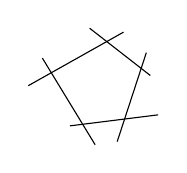
\begin{tikzpicture}[x=1cm,y=1cm]
\draw (-.22,.61)--(.99,1.29);
\draw (-.04,.96)--(.63,-.14);
\draw (.56,1.34)--(1.33,.74);
\draw (1.28,1.03)--(.91,-.10);
\draw (.31,.10)--(1.43,.24);
\end{tikzpicture}}
dans le \unsure{schéma} combinatoire de $C$. \deleted{\unsure{C'est suffisant},} \unsure{Réciproquemt|Réciproquement}, si $C$ n'a pas de pts \deleted{\unsure{doubles}} \inserted{multiples} ``multiplicatifs'', et si \deleted{\unsure{tous|les}} $C_i$ sont non \unsure{singuliers|singulières}, on voit par récurrence sur le nb des $C_i$ que $C$ \deleted{\unsure{est|$\to$}} $\operatorname{Pic}^{0}_{C/k}$ est une V.A.

On aura en tous cas
\margin{$g_i=\text{genre de }\widetilde{C}_i$}
\[
\begin{aligned}
g=\dim\operatorname{Pic}_{C/k}&=\sum g_i+\left(\sum_{\alpha}\mu_{\alpha}-c_{0}+1\right)\\
 &=\sum g_i+\deleted{\unsure{\mu_{\alpha}|\nu_{\alpha}}}\rho+\sigma
\end{aligned}
\]
$\rho=$ nb des cycles combinatoires, $+$ \unsure{somme|nombre} des \unsure{ints|ints.} des \unsure{multiplicités|multiplications} multiplicatives des $C_i$ [\unsure{cette} \unsure{dernière} $0$ si les $C_i$ non sing.]

$\sigma=$ somme des multiplicités additives des $P_{\alpha}$.
% archive sheet number: 150
